\scanpage{42}\mspage{41}
\uline{Prop} Soit $F'$ un raffinement de $F$. Conditions équivalentes

a) $F'$ est une subdivision

b) Il n'existe pas de $X\in M$ qui raffine $F$, et disjoint de $F'$

c) \deleted{Il n'existe pas \unsure{Ou bien} $\widetilde F'=\widetilde F$, sinon, \illegible{1} \unsure{de} \unsure{il} il n'existe pas de lieu du $F$} Il n'existe pas de lieu dans l'ombre $\widetilde F$, qui soit disjoint de $F'$ i.e. \inserted{(\deleted{par}\unsure{Cont|Cond|Corol} 6)} $\forall\deleted{\unsure{x}}x\unsure{\in|+}\widetilde F\setminus\widetilde F'$, $\exists\,y\in\widetilde F'$ tel que $x$ et $y$ \uline{non compatibles}, ou (positivement) : Si $x\in\widetilde F$ est compatible à tout élément de $\widetilde F'$, il est dans $\widetilde F'$.

\uline{Dém} $a\Longrightarrow b$, car si $X\in M$ raffine $F$ et est disjoint de $F'$, alors la figure $F\cup F_X$ est un raffinement de $F$, \unsure{strictmt|strictement} plus grand que $F'$,

$b)\Longrightarrow c)$ tautologique

$c)\Longrightarrow a)$ Si on avait, $F'\unsure{\subset|\in} \uline{F''}\not\ll F$, soit $X\in F''$, tel que $X\notin F'$, et soit $x\in\widetilde X^\circ$. Alors $x\in\widetilde F\setminus\widetilde F'$, et \deleted{je dis} que $x$ est compatible à $F'$ donc c) n'est pas vérifié.
% slanted
\margin{à vérifier}
\figure{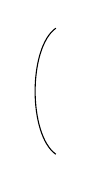
\begin{tikzpicture}[x=1cm,y=1cm]\draw (0.25,0.8) .. controls (-0.1,0.55) and (-0.1,-0.55) .. (0.25,-0.8);\end{tikzpicture}}

Mais on a utilisé que $x$ est compatible à $F'$, il faut un axiome pour l'assurer.

\uline{Cont} 7 Soient $X,\deleted{\unsure{X}}Y\in M$, \inserted{$X$ et $Y$ compatibles} $X\ne Y$. \inserted{(donc $\widetilde{\deleted{\unsure{Y}}X}^\circ\cap\widetilde Y^\circ=\varnothing$)} Alors tout $x\in\widetilde X^\circ$ est disjoint de tout $y\in\widetilde Y^\circ$ (ou, ce qui revient au $=$ par Cont 6, \deleted{tout} $x\in X^\circ$ est disjoint de $Y$)
\figure{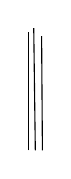
\begin{tikzpicture}[x=1cm,y=1cm]\draw (0,0)--(0,1.5);\draw (0.09,0)--(0.07,1.55);\draw (0.18,0)--(0.17,1.45);\end{tikzpicture}}

\uline{Cor. 1} Soient $F$ une figure, $F'$ une sous-figure et $X\in F\setminus F'$. Alors $\forall\,x\in X^\circ$ est \deleted{compatible} \inserted{disjoint} de $F'$.
